\documentclass[a4paper,fontsize=10.5pt,oneside,numbers=noenddot,parskip=half,headings=normal]{scrreprt}
\usepackage[T1]{fontenc}
\usepackage[utf8]{inputenc}
\usepackage{newtxtext,newtxmath}
\usepackage[margin=2cm,headheight=14pt,headsep=5mm,footskip=9mm]{geometry}
\usepackage{microtype,graphicx,booktabs,tabularx,array,float}
\usepackage[numbers,sort&compress]{natbib}
\usepackage{caption,chngcntr,fancyhdr,enumitem}
\usepackage[hidelinks]{hyperref}
\counterwithout{figure}{chapter}
\counterwithout{table}{chapter}
\setcounter{tocdepth}{0}
\setlength{\parindent}{0pt}
\setlength{\emergencystretch}{1em}
\linespread{1.06}
\captionsetup{font=small,labelfont=bf,skip=5pt}
\setlength{\textfloatsep}{9pt}
\setlength{\intextsep}{8pt}
\renewcommand{\arraystretch}{1.16}
\RedeclareSectionCommand[beforeskip=0pt,afterskip=10pt]{chapter}
\RedeclareSectionCommand[beforeskip=10pt,afterskip=5pt]{section}
\RedeclareSectionCommand[beforeskip=7pt,afterskip=3pt]{subsection}
\setkomafont{chapter}{\normalfont\sffamily\LARGE\bfseries}
\setkomafont{section}{\normalfont\sffamily\large\bfseries}
\setkomafont{subsection}{\normalfont\sffamily\normalsize\bfseries}
\pagestyle{fancy}
\fancyhf{}
\fancyhead[L]{\small\sffamily COMP90072 \;|\; Sandpile project}
\fancyhead[R]{\small\sffamily Draft report}
\fancyfoot[C]{\thepage}
\renewcommand{\headrulewidth}{0.3pt}
\renewcommand{\chapterpagestyle}{fancy}
\newcolumntype{Y}{>{\raggedright\arraybackslash}X}
\hypersetup{pdftitle={Two-dimensional sandpile dynamics: avalanche statistics and random redistribution},pdfauthor={Zhang Wenbo},pdfsubject={COMP90072 draft coursework report}}
\begin{document}

\begin{titlepage}
\thispagestyle{empty}
{\sffamily\large COMP90072\par}
{\sffamily The Art of Scientific Computing\par}
\vspace{1.1cm}
{\sffamily\bfseries\fontsize{27}{33}\selectfont Two-dimensional\par sandpile dynamics\par}
\vspace{0.55cm}
{\sffamily\fontsize{17}{23}\selectfont Avalanche statistics and\par random redistribution\par}
\vspace{0.8cm}
\rule{\textwidth}{0.5pt}
\vspace{0.5cm}
{\large Draft coursework report\par}
\vspace{0.8cm}
\begin{tabular}{@{}ll}
Student name: & Zhang Wenbo \\[0.55cm]
Student ID: & 1873749 \\[0.55cm]
Date: & 8 October 2026
\end{tabular}
\vfill
\section*{Abstract}
I studied avalanches in the two-dimensional Bak--Tang--Wiesenfeld model using open grids of width 16, 32 and 64. Each setting has three runs with 20,000 recorded grain additions after burn-in. The mean height rises from 2.0465 to 2.1040 across these sizes, while the mean run-level 99th percentile of nonzero toppling counts rises from 192.66 to 4,329.51. I also compared deterministic redistribution with a rule in which each outgoing grain independently chooses a direction. At width 32, the random rule gives more topplings per avalanche on average, but a smaller mean area and radius. The same saved data support the figures and tables throughout this draft. The main remaining questions concern how much can be inferred from the tail fits and how best to explain the role of the boundary.

\small
Working draft for feedback. The revision questions are listed in Appendix A.
\normalsize
\end{titlepage}

\pagenumbering{arabic}

\chapter{Introduction}\label{ch:intro}
The starting question is how a single added grain can produce such different responses in the same system. Sometimes nothing topples; at other times the disturbance spreads across much of the grid. I use the sandpile model and questions in the course handout, including the extension that assigns an independent random direction to each outgoing grain~\cite{course}.

The BTW model was introduced as an example of self-organised criticality~\cite{bak1987}. It combines slow external driving with rapid local relaxation. A site responds only when its height reaches a threshold, and its response can push neighbouring sites over their thresholds. This gives a route from a small local change to a much larger event. The separation of timescales is imposed directly here: another grain is added only after the preceding avalanche has ended.

\section{Questions and scope}
I kept the three questions from the revised project plan: how the pile approaches a steady statistical regime, how its avalanche measurements change with grid width, and what changes when the outgoing directions become random. The implementation checks come first because even a small boundary error would affect the later statistics. This draft brings the model, the checks and the main numerical comparisons together.

The numerical study uses $L=16,32,64$ for BTW and $L=32$ for the extension. This scale is manageable with a short Python program and allows repeated runs and diagnostic checks. I expected the height to rise from an empty grid and eventually fluctuate within a narrower range. An initial guess of 1.5 came from assuming equal frequencies of the four stable heights. That assumption is tested explicitly in Chapter~\ref{ch:results}. For the extension, the preserved input and average outgoing transfer suggested similar long-run mass balance. The direction of the changes in avalanche geometry was left to the comparison.

\section{Scale invariance and the finite-grid setting}\label{sec:scale}
Suppose a nonzero statistical function retains its shape under a continuous range of rescalings. A homogeneous representation is
\begin{equation}
 f(bx)=b^{-\tau}f(x).
\end{equation}
For differentiable $f$, differentiating with respect to $b$ at $b=1$ gives $xf'(x)=-\tau f(x)$. Integration yields $f(x)=Cx^{-\tau}$. A power law therefore has no characteristic scale within the range where this relation holds. Discrete rescaling alone is weaker and may allow log-periodic corrections. For a mass function with tail $p(s)\propto s^{-\tau}$ and $\tau>1$, the corresponding far-tail complementary cumulative distribution has exponent $1-\tau$ under the usual tail approximation.

The lattice spacing sets a minimum length, while the finite grid bounds the area and propagation radius. Any apparent scaling must be assessed within those limits. I use distribution curves and several lower fitting thresholds to see how far a simple power-law description can be taken.

\section{Why the boundary matters}\label{sec:boundary}
A finite closed grid gains one grain at every driving step. Stable configurations hold at most $3L^2$ grains, so continued conservative driving eventually prevents complete stabilisation. Open boundaries provide an outlet. An infinite grid requires a different specification: a uniform positive selection probability cannot be assigned to every site of $\mathbb Z^2$. Driving a finite subset is possible, but outward transport from a finite observation window leaves grains elsewhere in the infinite system. Statements about its limiting state also require an initial configuration and a defined order of limits. I therefore use the finite open model for the numerical work.

\chapter{Model and stabilisation theory}\label{ch:model}
\section{Local rule and recorded quantities}\label{sec:rule}
The state is an $L\times L$ array of nonnegative integer heights, initially zero. A uniformly selected site receives one grain. Whenever $h(i,j)\geq4$, that site loses four grains and sends one in each of the four nearest-neighbour directions. A grain directed outside the grid is removed. This is repeated until all heights are below four. Edge and corner sites retain the same threshold. A driving step counts one addition and its complete relaxation.

If $u(x)$ is the number of topplings at site $x$ during that relaxation and $x_0$ is the addition site, the recorded quantities are
\begin{equation}\label{eq:metrics}
 s=\sum_xu(x),\qquad a=\#\{x:u(x)>0\},\qquad
 r=\max_{u(x)>0}\lVert x-x_0\rVert_2,\qquad H=\frac{1}{L^2}\sum_xh(x).
\end{equation}
Boundary loss $d$ counts grains that leave during the same relaxation. Lattice spacing is one. The radius directly measures how far the disturbance reaches and is inexpensive to calculate from the toppled sites. A step without a toppling has $s=a=d=r=0$. A one-site avalanche also has $r=0$, so the event definition is always $s>0$. Repeated topplings increase $s$ while contributing only once to $a$.

\section{Toppling matrix and dissipation}\label{sec:matrix}
The Abelian formulation gives a useful way to express the update and study its dependence on processing order~\cite{dhar1999}. I use the handout's negative-diagonal convention: row $x$ gives the increment caused by toppling at $x$,
\begin{equation}\label{eq:delta}
\Delta(x,y)=\begin{cases}-4,&x=y,\\1,&x,y\text{ are nearest neighbours within the grid},\\0,&\text{otherwise}.\end{cases}
\end{equation}
Its conditions have direct interpretations (Table~\ref{tab:matrix}). Symmetry describes the undirected transfer in this model; directed dissipative sandpiles can be defined as well.
\begin{table}[H]
\centering\small
\caption{Meaning of the toppling-matrix conditions.}\label{tab:matrix}
\begin{tabularx}{\linewidth}{@{}p{5.7cm}Y@{}}\toprule
Condition & Meaning \\\midrule
$\Delta(x,y)=\Delta(y,x)\geq0$, $x\ne y$ & A toppling supplies nonnegative amounts to other sites, with symmetric transfer.\\
$\Delta(x,x)<0$ & It removes grains from its own site; the threshold is $-\Delta(x,x)$.\\
$\sum_y\Delta(x,y)\leq0$ & It conserves or reduces total mass.\\
$\sum_{x,y}\Delta(x,y)<0$ & At least one site is dissipative.\\\bottomrule
\end{tabularx}
\end{table}
For an interior site the row sum is zero; at a non-corner edge it is $-1$, and at a corner it is $-2$. The total is $-4L$ for $L\geq2$. A single-site grid has matrix $[-4]$. With this sign convention, the instability condition is $h(x)\geq-\Delta(x,x)=4$; the printed sign in the handout's Equation (6) is inconsistent with its stated rule.

Every site must also have a path to a dissipative site. The four conditions alone do not guarantee this on a disconnected graph. For example,
\begin{equation}
\Delta=\begin{pmatrix}-1&1&0\\1&-1&0\\0&0&-1\end{pmatrix}
\end{equation}
satisfies them, but a grain at site 1 can move indefinitely between sites 1 and 2 under the threshold-one rule. The open square grid has the required accessibility.

\clearpage
\section{Why legal relaxation has a unique outcome}\label{sec:abelian}
The following argument separates termination from uniqueness. It follows the finite-graph treatment and least-action reasoning described by J\'arai~\cite{jarai2018}. During relaxation the initial mass is finite, no new grains arrive, and all heights remain nonnegative.

\subsection{Termination}
Suppose a legal relaxation contains infinitely many topplings. Since the grid has finitely many sites, at least one site topples infinitely often. Each of its neighbours then receives infinitely many grains. A neighbour that toppled only finitely often would accumulate unbounded height, contradicting the finite upper bound on total mass. Thus every neighbour must also topple infinitely often. Following a path through the connected grid reaches a boundary site. Its repeated topplings would lose infinitely many grains, again contradicting the finite initial mass. The relaxation must end.

\subsection{Exchanging two legal topplings}
Let $\Delta_x$ be row $x$ viewed as an increment vector. An executed toppling gives $T_xh=h+\Delta_x$. If two sites $x$ and $y$ are both unstable, toppling either cannot reduce the height of the other. Both orders remain legal, and
\begin{equation}\label{eq:commute}
 T_yT_xh=h+\Delta_x+\Delta_y=T_xT_yh.
\end{equation}
The legality condition matters for a conditional operation that does nothing at a stable site. Starting from $\left(\begin{smallmatrix}3&4\\0&0\end{smallmatrix}\right)$, select the upper-left site $x$ and upper-right site $y$. Applying $T_x$ then $T_y$ gives $\left(\begin{smallmatrix}4&0\\0&1\end{smallmatrix}\right)$; applying $T_y$ then $T_x$ gives $\left(\begin{smallmatrix}0&1\\1&1\end{smallmatrix}\right)$. In the first order, $x$ still needs to topple. Completing the relaxation gives the same final state. This resolves the ambiguity in treating every conditional operation as freely interchangeable.

\subsection{Uniqueness of the complete relaxation}
Take two complete legal stabilisations from the same initial state $h$, with total site-level toppling counts $u(x)$ and $v(x)$. Follow the first sequence and suppose a site's count is about to exceed $v$ for the first time. Just before that toppling at $x$, the partial counts $n$ satisfy $n(x)=v(x)$ and $n(y)\leq v(y)$ for every other site. The current height at $x$ is therefore
\begin{align}
 h(x)+\Delta(x,x)n(x)+\sum_{y\ne x}\Delta(y,x)n(y)
 &\leq h(x)+\Delta(x,x)v(x)+\sum_{y\ne x}\Delta(y,x)v(y)\notag\\
 &=h_{\mathrm{final},v}(x)<4.\label{eq:leastaction}
\end{align}
The inequality uses the nonnegative off-diagonal entries. The proposed toppling would be illegal, which contradicts its selection. Hence $u\leq v$. Reversing the two sequences gives $v\leq u$, so $u=v$ and
\begin{equation}\label{eq:final}
 h_{\mathrm{final}}=h+\Delta^{\mathsf T}u
\end{equation}
is unique. This establishes both the final heights and the number of topplings at every site. It justifies choosing a convenient legal processing order in the program.

The associated addition-and-stabilisation chain, with positive driving probability at every site, has a single recurrent communicating class. Its stationary measure is uniform on recurrent configurations. On that class, the process is ergodic for time averages under the stated driving conditions. The time and ensemble comparison in Section~\ref{sec:ensemble} uses this setting. Configurations generated by independently selecting heights from $0,1,2,3$ form a different sample space.

\chapter{Computational methods}\label{ch:methods}
\section{A candidate-list relaxation algorithm}\label{sec:algorithm}
The core program uses NumPy integer arrays and a double-ended queue. Each drive begins by adding a grain and placing its site in the candidate list. The last candidate is removed first. Its height is checked again, since a listed site need not still require a toppling. A legal toppling updates four neighbours, the site-level count array, and the boundary loss. A neighbour is added when it first reaches height four. The source is added again if it remains unstable. Figure~\ref{fig:flow} shows the complete loop.

This arrangement avoids scanning the entire grid to choose each next toppling. The local work is proportional to the number of processed candidates and four transfers per executed toppling. Computing the recorded area, radius and full-grid checks adds array work of order $L^2$ per addition. That cost is acceptable for the selected sizes and keeps the implementation easy to inspect. Only one height grid and the current toppling-count array are needed during relaxation; the saved trajectory stores five scalar measurements per driving step.
\begin{figure}[H]
\centering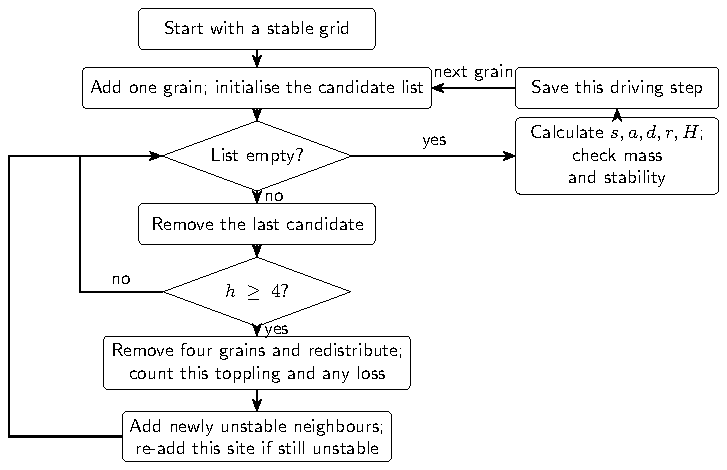
\includegraphics[width=0.75\linewidth]{figures/flowchart.pdf}
\caption{Candidate-list algorithm for one grain addition and complete relaxation. The same loop handles both rules; only the choice of outgoing directions changes. A new driving step starts after the candidate list is empty and the checks have passed.}\label{fig:flow}
\end{figure}
\section{Checks before collecting statistics}\label{sec:checks}
For every simulated step the program checks the exact integer identity
\begin{equation}\label{eq:mass}
 M_{t+1}=M_t+1-d_t,
\end{equation}
as well as nonnegative stable heights and $a\leq s$. Local tests cover centre, edge and corner topplings. A separate synchronous array algorithm provides a cross-check on the candidate-list implementation. All 1,024 additions to stable $2\times2$ grids, together with 100 random unstable $8\times8$ configurations, produced identical final heights, site-level toppling counts and loss under last-in-first-out, first-in-first-out and synchronous processing.

The 1,124 comparisons passed again during report preparation. A read-only audit of all 782,220 saved steps found zero mass-balance residual. These tests support the implementation; the complete mathematical statement about processing order is established in Section~\ref{sec:abelian}.

\clearpage
\section{Sampling design and statistical summaries}\label{sec:sampling}
Each run starts empty. The initial burn-in is $B=\max(5000,10L^2)$, followed by 20,000 recorded additions. Three seeds are used per main setting. Burn-in is checked through height windows, comparisons of the two halves of the recorded phase, and an additional doubled-burn-in experiment at $L=32$ (Table~\ref{tab:design}).
\begin{table}[H]
\centering\small
\caption{Experiments included in the saved data. Recorded additions exclude burn-in.}\label{tab:design}
\begin{tabularx}{\linewidth}{@{}Yrrrr@{}}\toprule
Experiment & $L$ & Burn-in & Recorded & Runs\\\midrule
BTW &16&5,000&20,000&3\\
BTW &32&10,240&20,000&3\\
BTW &64&40,960&20,000&3\\
Random redistribution &32&10,240&20,000&3\\
Doubled burn-in, each rule &32&20,480&20,000&3 each\\
Independent BTW ensemble &16&5,000&1&20\\\bottomrule
\end{tabularx}
\end{table}
The main experiments contain 240,000 recorded additions and 99,143 nonzero avalanches. Summary means and quantiles are calculated within each run before taking the mean and sample standard deviation across the three runs. Distribution curves pool the three equal-length records. Spearman correlations use all events with $s>0$, including events with zero loss or radius.

For logarithmic plots I use the exact positive-value CCDF, $P(X\geq x\mid X>0)$, separately for each variable. Zero frequencies remain in the full data. The exploratory fitting calculation follows the discrete likelihood formulation of Clauset and colleagues~\cite{clauset2009}:
\begin{equation}\label{eq:fit}
 p(s\mid s\geq s_{\min})=\frac{s^{-\alpha}}{\zeta(\alpha,s_{\min})},\qquad
 -\ell(\alpha)=n\log\zeta(\alpha,s_{\min})+\alpha\sum_{i=1}^{n}\log s_i.
\end{equation}
I minimise this expression for $\alpha>1$ at six fixed thresholds. The output contains the tail sample size and the maximum empirical-to-fitted CDF distance (KS distance). No bootstrap goodness-of-fit test or comparison with alternative distributions was performed. The site-level count array also gives a spatial check on the avalanche measurements (Figure~\ref{fig:peak}).
\begin{figure}[H]
\centering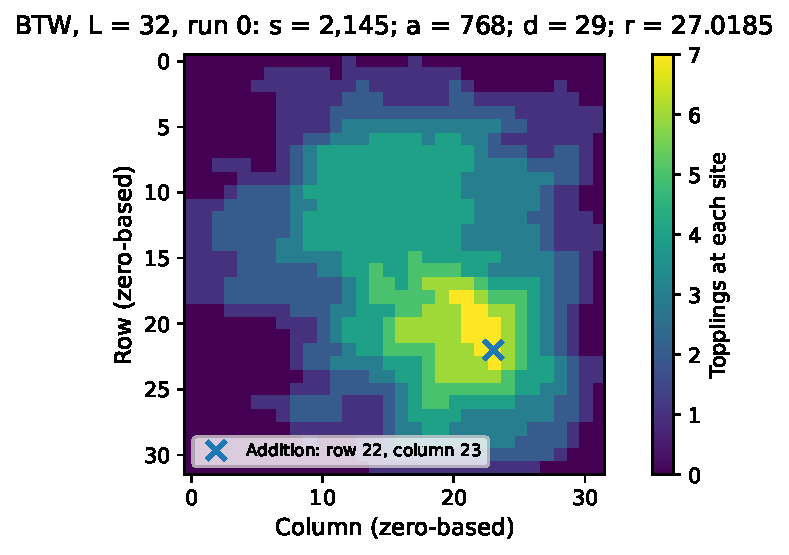
\includegraphics[width=0.72\linewidth]{figures/peak.pdf}
\caption{Site-level topplings for the largest recorded avalanche in BTW $L=32$, run 0. It occurs at post-burn-in addition 13,646 and has $s=2{,}145$, $a=768$, $d=29$ and $r=27.0185$. The cross marks zero-based row 22, column 23; a site topples at most seven times. This is a selected large event from one run.}\label{fig:peak}
\end{figure}

\chapter{Results for the BTW model}\label{ch:results}
\section{Loading, mean height and the stationary regime}\label{sec:height}
The initial height guess was $(0+1+2+3)/4=1.5$. It assumes equal frequencies of the four stable heights and ignores the dependence created by redistribution. The measured averages are all higher. Figure~\ref{fig:heighttrace} shows the early loading and later fluctuations for one run; Figure~\ref{fig:heightmeans} compares the averages across all three runs per setting.

For the infinite square lattice, the exact stationary BTW mean is $17/8=2.125$ under the present $0$--$3$ height convention. The result is commonly written as $25/8$ with heights $1$--$4$~\cite{poghosyan2011}. The finite-grid averages in Figure~\ref{fig:heightmeans} increase from 2.0465 at $L=16$ to 2.1040 at $L=64$, moving towards that benchmark. This is consistent with the decreasing relative importance of boundary sites.
\begin{figure}[H]
\centering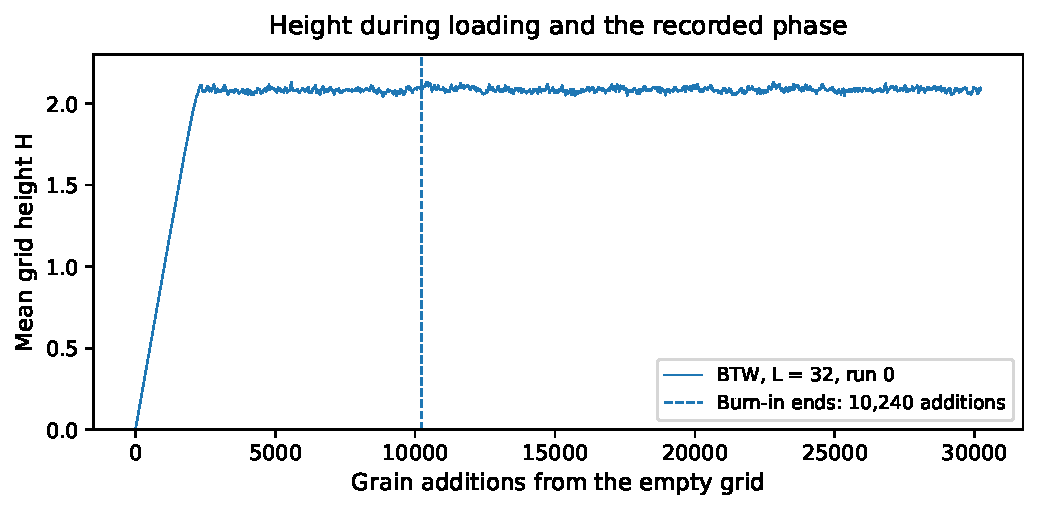
\includegraphics[width=0.81\linewidth]{figures/height_trace.pdf}
\caption{Mean height in BTW $L=32$, run 0, from the empty grid through the recorded phase. The vertical line marks the end of 10,240 burn-in additions. Every 25th step is displayed; all steps are used in the calculations. This single trajectory is distinct from the three-run summaries below.}\label{fig:heighttrace}
\end{figure}
\begin{figure}[H]
\centering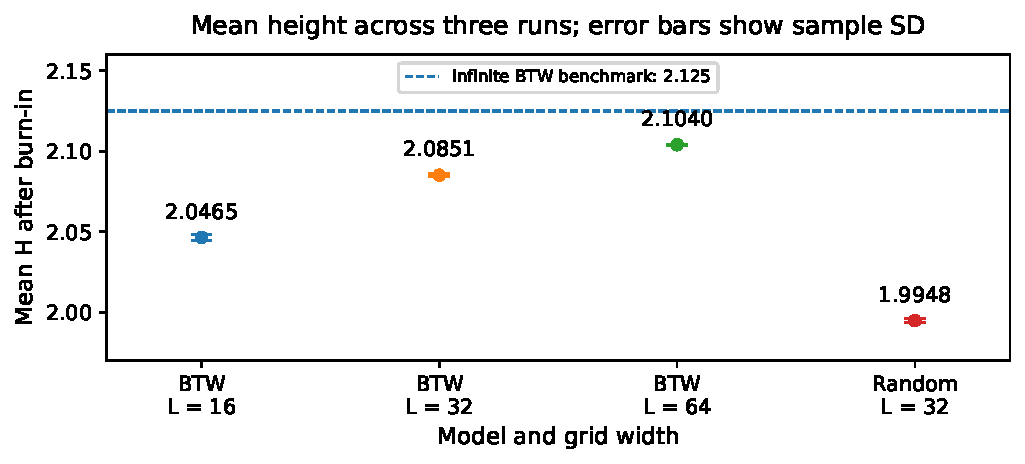
\includegraphics[width=0.81\linewidth]{figures/height_means.pdf}
\caption{Mean post-burn-in height across three runs per setting. The labels are rounded to four decimal places; error bars show run-to-run sample SD. The random-rule value is included for the later comparison. The dashed benchmark applies to infinite-lattice BTW.}\label{fig:heightmeans}
\end{figure}
A stable configuration means $h<4$ everywhere. Statistical stationarity concerns distributions that remain unchanged under a shift of observation time. The late trajectory still changes from one drive to the next, while its height stays in a much narrower range. Here steady state refers to long-run statistics, while thermodynamic equilibrium excludes this sustained driving-and-loss process. Grains continue to enter and leave the system. The height plateau is a useful diagnostic, with the burn-in sensitivity in Section~\ref{sec:draftlimits} providing a further check.

\clearpage
\section{Time sampling and independent ensembles}\label{sec:ensemble}
Time sampling follows successive states of one system, so neighbouring observations can be correlated. Ensemble sampling draws observations from separately driven systems. The two estimates need sufficient sampling of the relevant recurrent states to be comparable. A short run, an initial transient or strong time correlation can create visible differences.

For BTW at $L=16$, I took the 20,000 post-burn-in heights from run 0 and divided them into 40 non-overlapping blocks of 500 steps. Their mean is 2.044285. I estimated a standard error from the block means, treating them as approximately independent. The comparison ensemble consists of 20 independently seeded systems, each observed after 5,001 additions from an empty grid. Its mean is 2.055664.
\begin{figure}[H]
\centering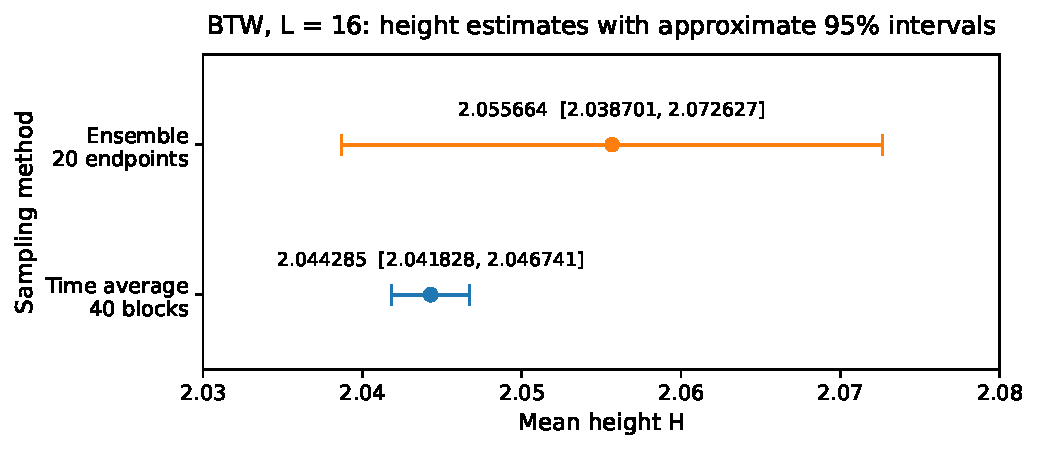
\includegraphics[width=0.91\linewidth]{figures/time_ensemble.pdf}
\caption{Time and ensemble estimates for mean height at $L=16$. Horizontal intervals use Student-$t$ multipliers. The time interval treats 40 block means as approximately independent; the ensemble interval uses 20 independent endpoints. Numerical values are also given in Table~\ref{tab:ensemble}.}\label{fig:ensemble}
\end{figure}
\begin{table}[H]
\centering\small
\caption{Values used in Figure~\ref{fig:ensemble}. These are approximate confidence intervals, unlike the three-run SD bars used elsewhere.}\label{tab:ensemble}
\begin{tabularx}{\linewidth}{@{}Yrrl@{}}\toprule
Estimate & Mean $H$ & Standard error & Approximate 95\% interval\\\midrule
Time: 40 block means &2.044285&0.001215&[2.041828, 2.046741]\\
Ensemble: 20 endpoints &2.055664&0.008105&[2.038701, 2.072627]\\\bottomrule
\end{tabularx}
\end{table}
The time estimate lies within the much wider ensemble interval (Figure~\ref{fig:ensemble}). The difference is compatible with the sampling uncertainty of these 20 endpoints. The check concerns one observable at one grid width; it does not establish equal sampling accuracy for the avalanche tail.

The theoretical setting in Section~\ref{sec:abelian} supports relating long-run time averages to the stationary ensemble on the recurrent class. It does not give uniform sampling over every stable configuration. A burning test in the saved analysis identified all 32 deterministic final configurations as recurrent. This confirms their class membership, while mixing within that class remains a separate issue.

Periodicity also deserves care. On a one-site grid, successive heights follow $1,2,3,0$ repeatedly. Its long-run mean is well defined, but its distribution at a fixed time from a fixed starting state continues to cycle. The numerical test includes this small example. For the larger runs, the block and burn-in diagnostics provide a practical assessment of the available stationary-window estimates.

\clearpage
\section{Avalanche distributions and grid width}\label{sec:distributions}
\subsection{Topplings and area}
Both toppling count and area have broad, right-skewed distributions (Figures~\ref{fig:sccdf} and~\ref{fig:accdf}). Larger grids extend the range of large events. The average run-level 99th percentile of $s$, conditional on an avalanche, is 192.66, 942.57 and 4,329.51 at $L=16,32,64$ respectively (Table~\ref{tab:main}). These quantiles are calculated within runs; the plotted CCDFs pool the runs.
\begin{table}[H]
\centering\small
\caption{Main BTW size summaries. Entries are means $\pm$ sample SD of three run-level estimates. The last column averages the three separately calculated event quantiles.}\label{tab:main}
\begin{tabular}{@{}lrrr@{}}\toprule
Setting & $P(s>0)$, percent & Mean $s$, all additions & 99th percentile, $s>0$\\\midrule
BTW $L=16$&$40.982\pm0.319$&$11.3331\pm0.0491$&$192.66\pm6.04$\\
BTW $L=32$&$41.883\pm0.201$&$40.5030\pm0.2150$&$942.57\pm11.17$\\
BTW $L=64$&$43.175\pm0.157$&$153.1406\pm0.4993$&$4329.51\pm153.25$\\\bottomrule
\end{tabular}
\end{table}
\begin{figure}[H]
\centering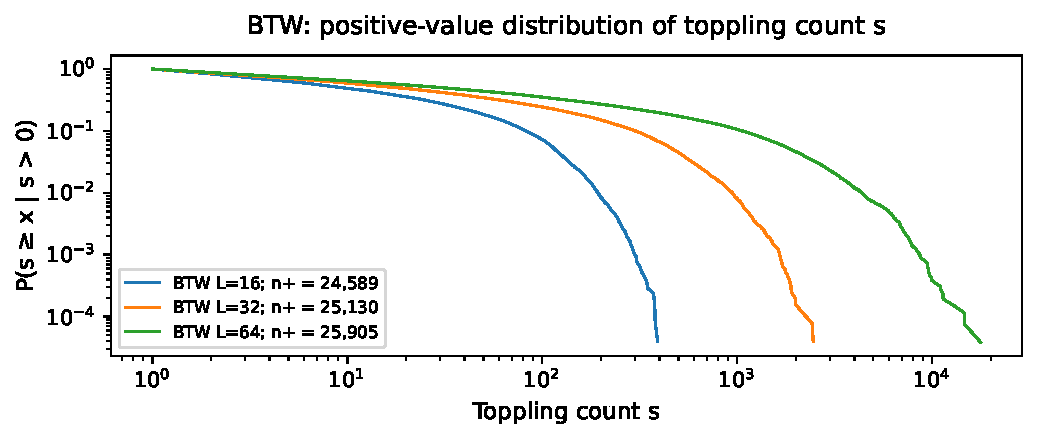
\includegraphics[width=0.91\linewidth]{figures/ccdf_btw_s.pdf}
\caption{Positive-value CCDF of the number of topplings. Each curve pools three runs, each with 20,000 recorded additions. The legend gives the number of nonzero observations. The larger-$L$ curves extend to substantially greater toppling counts.}\label{fig:sccdf}
\end{figure}
\begin{figure}[H]
\centering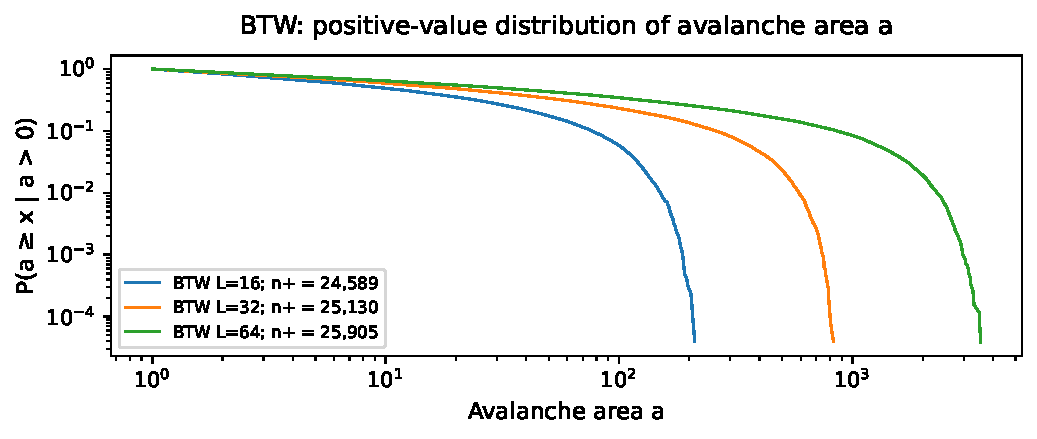
\includegraphics[width=0.91\linewidth]{figures/ccdf_btw_a.pdf}
\caption{Positive-value CCDF of avalanche area for the same runs. The positive sample counts equal those for $s$, because an avalanche has at least one toppled site. Area is bounded by $L^2$; repeated topplings do not add new sites.}\label{fig:accdf}
\end{figure}
The similar ordering of these curves is expected because avalanches with many topplings often visit more sites. Their numerical values still differ. For example, the event in Figure~\ref{fig:peak} has 2,145 topplings spread over 768 sites.

\clearpage
\subsection{Boundary loss and propagation radius}
Loss is zero for many additions, including some that trigger avalanches. Radius can also vanish during a one-site avalanche. Table~\ref{tab:zeros} gives these zero frequencies. Figures~\ref{fig:dccdf} and~\ref{fig:rccdf} show only the positive part of each variable, so they have different sample sizes and conditional denominators.
\begin{figure}[H]
\centering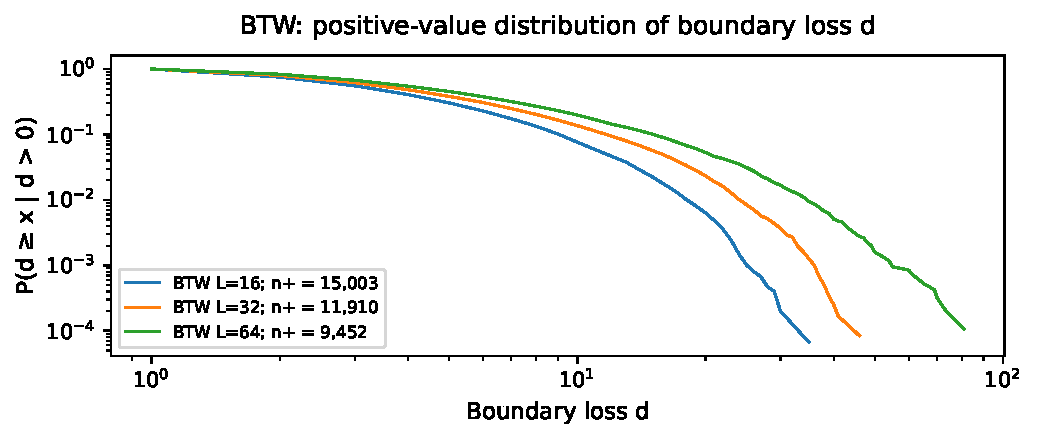
\includegraphics[width=0.85\linewidth]{figures/ccdf_btw_d.pdf}
\caption{Boundary loss conditional on $d>0$. Larger grids have fewer loss-producing additions in these records (Table~\ref{tab:zeros}), although positive loss events can be larger. Mean loss over all additions stays close to one.}\label{fig:dccdf}
\end{figure}
\begin{figure}[H]
\centering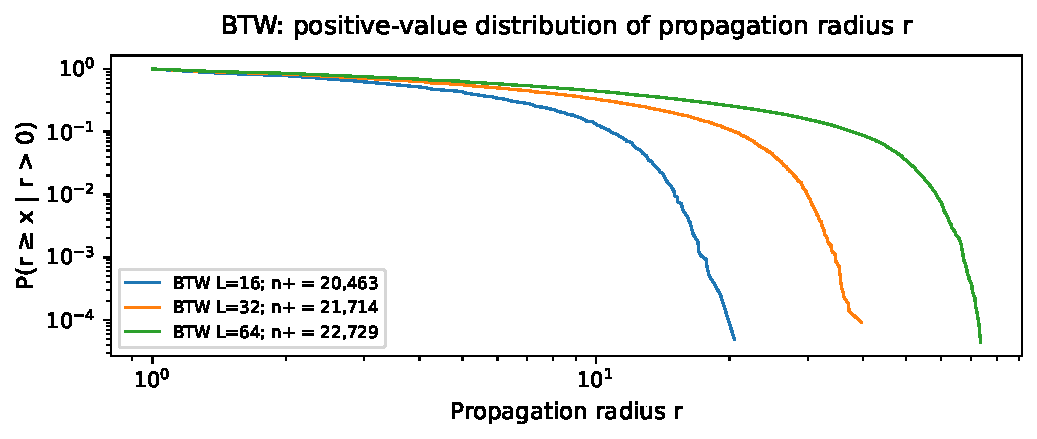
\includegraphics[width=0.85\linewidth]{figures/ccdf_btw_r.pdf}
\caption{Propagation radius conditional on $r>0$. Distances are Euclidean with unit lattice spacing. The bound is $r\leq\sqrt{2}(L-1)$. The outward shift with $L$ reflects the larger available spatial extent.}\label{fig:rccdf}
\end{figure}
\begin{table}[H]
\centering\small
\caption{Zero-valued additions, as percentages of all 60,000 recorded additions per setting. The random setting is included for Chapter~\ref{ch:extension}.}\label{tab:zeros}
\begin{tabular}{@{}lrrrr@{}}\toprule
Model & $s=0$ & $a=0$ & $d=0$ & $r=0$\\\midrule
BTW $L=16$&59.018&59.018&74.995&65.895\\
BTW $L=32$&58.117&58.117&80.150&63.810\\
BTW $L=64$&56.825&56.825&84.247&62.118\\
Random $L=32$&60.802&60.802&84.793&65.622\\\bottomrule
\end{tabular}
\end{table}

The positive loss and radius distributions are also right-skewed. Loss includes a substantial probability at zero, while radius is restricted to distances available on the lattice. A symmetric Gaussian would miss these features. I applied the exploratory power-law fit to toppling count, whose discrete tail can be specified directly.

\clearpage
\section{Relationships between the measurements}\label{sec:correlation}
Before calculating the correlations, I expected toppling count, area and radius to be positively related. An avalanche that keeps spreading usually both visits more sites and performs more topplings. Loss should have a less direct relationship because the location of the initial addition and contact with the boundary also matter.

The measurements support this expectation. In BTW at $L=32$, the Spearman correlation of $s$ with $a$ is 0.9992, and that of $s$ with $r$ is 0.9836 (Figure~\ref{fig:corr}). The correlation of $s$ with loss is lower, at 0.5532. Table~\ref{tab:corr} shows every pair for this grid width and the random extension.
\begin{figure}[H]
\centering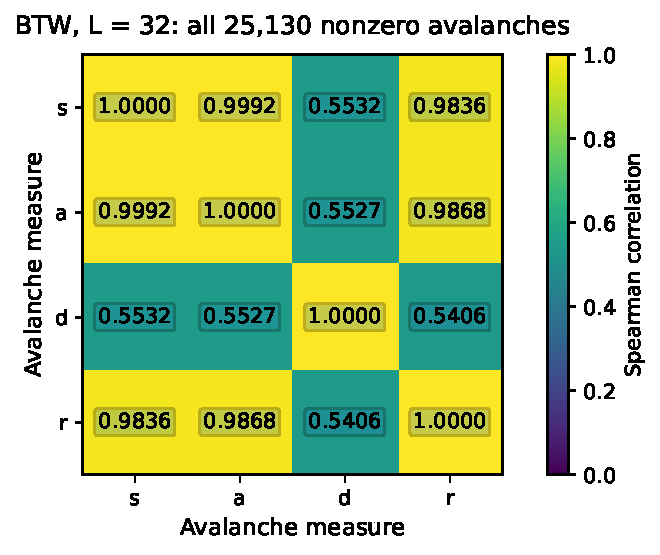
\includegraphics[width=0.71\linewidth]{figures/correlation.pdf}
\caption{Spearman correlations among all 25,130 nonzero BTW avalanches at $L=32$, pooled across three runs. Zero loss and zero radius are retained. Displayed values use four decimal places and match the BTW column of Table~\ref{tab:corr}.}\label{fig:corr}
\end{figure}
\begin{table}[H]
\centering\small
\caption{Descriptive rank correlations at $L=32$. The random model contributes 23,519 nonzero avalanches.}\label{tab:corr}
\begin{tabular}{@{}lrr@{}}\toprule
Pair & BTW & Random redistribution\\\midrule
$s,a$&0.9992&0.9986\\
$s,d$&0.5532&0.4949\\
$s,r$&0.9836&0.9798\\
$a,d$&0.5527&0.4942\\
$a,r$&0.9868&0.9835\\
$d,r$&0.5406&0.4827\\\bottomrule
\end{tabular}
\end{table}
A high rank correlation describes the ordering of observations. It allows a substantial difference in their magnitudes: $a\leq s$, and repeated topplings can make the gap large. This becomes particularly relevant to the random extension. The weaker loss correlations fit the additional role of the boundary, although the correlation matrix alone cannot separate the contributions of initial position and avalanche geometry.

The estimates use every nonzero event in the chosen records. Since events are generated along trajectories, I use these coefficients descriptively and do not attach independence-based significance tests. The accompanying analysis package also retains the original scatter plots and the correlations for the other BTW grid widths.

\clearpage
\section{What the power-law fits establish}\label{sec:fits}
The fits in Equation~\eqref{eq:fit} were calculated at $s_{\min}=5,10,20,50,100,200$. Figure~\ref{fig:fits} shows the two $L=32$ models. For BTW, the fitted exponent rises from 1.4141 at threshold 5 to 2.4372 at threshold 200. The random model also shows threshold dependence. There is no stable estimate across this full range of lower cutoffs.
\begin{figure}[H]
\centering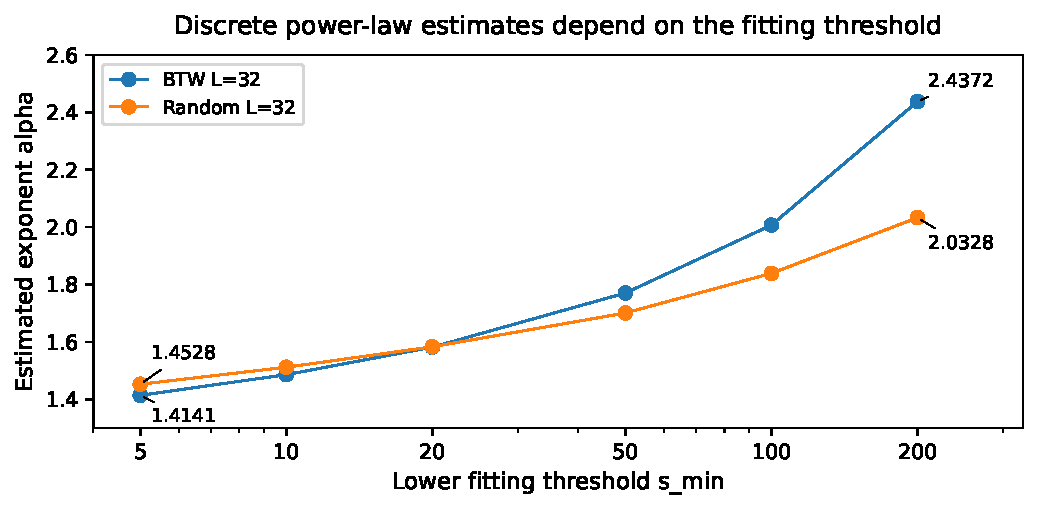
\includegraphics[width=0.91\linewidth]{figures/fit_threshold.pdf}
\caption{Exploratory discrete maximum-likelihood estimates for the two $L=32$ settings. Points use the same six thresholds. The labels identify the endpoint estimates; the line segments simply join the estimates. No confidence intervals are claimed.}\label{fig:fits}
\end{figure}
\begin{table}[H]
\centering\small
\caption{Fits at $s_{\min}=20$ for all four main settings. KS is the maximum CDF distance and has no p-value interpretation here. All 24 fitted rows are supplied in the data package.}\label{tab:fits}
\begin{tabular}{@{}lrrr@{}}\toprule
Setting & Tail observations & $\widehat\alpha$ & KS distance\\\midrule
BTW $L=16$&8,776&1.9746&0.1319\\
BTW $L=32$&12,173&1.5819&0.1349\\
BTW $L=64$&14,345&1.4170&0.1322\\
Random $L=32$&9,390&1.5833&0.0864\\
\bottomrule
\end{tabular}
\end{table}
The finite-grid CCDFs bend towards their largest events, so progressively raising the lower threshold changes the portion of the distribution being fitted. An unbounded power law cannot represent every aspect of a finite-grid distribution. Known difficulties with simple finite-size scaling in the Abelian sandpile provide further reason to interpret a single fitted slope cautiously~\cite{demenech1998}.

The present calculation estimates parameters and records a discrepancy measure. It provides no bootstrap goodness-of-fit probability and no likelihood-ratio comparison against a truncated power law or a lognormal model. I therefore retain the visible distribution shapes and the threshold dependence as the main results of this part of the project.


\chapter{Random redistribution extension}\label{ch:extension}
\section{Changing the outgoing directions}\label{sec:random}
The extension keeps the threshold at four. At each toppling, four grains leave the source, and each independently chooses up, down, left or right with probability $1/4$. Several may reach the same neighbour. A direction outside the grid remains a loss event; it is not redrawn. The expected transfer in each direction is still one grain, although its realised value fluctuates.

The comparison uses $L=32$ and three repeats per rule. Within a repeat, both models receive exactly the same recorded addition positions. Burn-in positions, recorded positions and random outgoing directions have separate random streams. The direction stream continues through burn-in. Thus the doubled-burn-in comparison preserves the later drive positions while allowing a different internal random history.
\begin{figure}[H]
\centering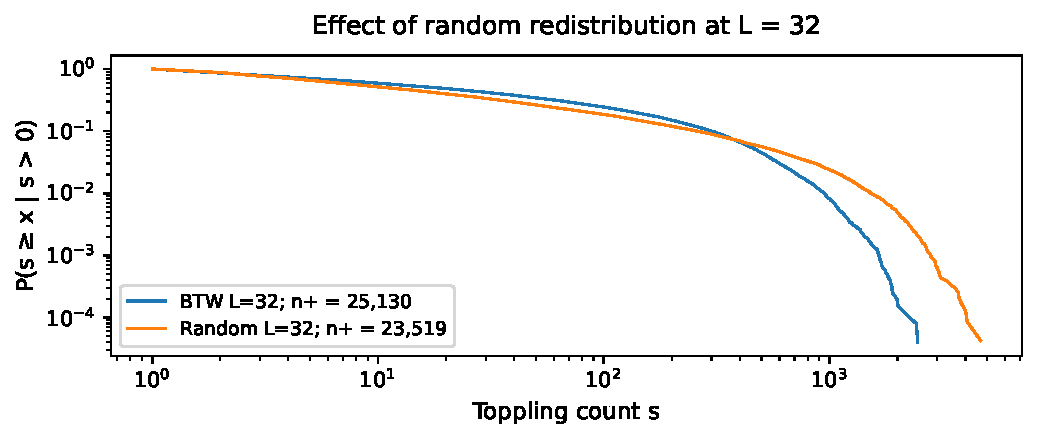
\includegraphics[width=0.87\linewidth]{figures/random_ccdf.pdf}
\caption{Positive toppling-count distributions at $L=32$, pooling the three runs per rule. The curves cross, so their ordering depends on the threshold examined. Table~\ref{tab:random} reports specific run-level means and quantiles, with their conditioning stated explicitly.}\label{fig:random}
\end{figure}
\begin{table}[H]
\centering\small
\caption{Comparison at $L=32$. Each entry is the mean $\pm$ sample SD across three runs. Probabilities use the 0--1 scale. ``Event'' means an addition with $s>0$.}\label{tab:random}
\begin{tabularx}{\linewidth}{@{}Yrr@{}}\toprule
Quantity & BTW & Random redistribution\\\midrule
Mean height $H$&$2.0851\pm0.0011$&$1.9948\pm0.0011$\\
$P(s>0)$, all additions&$0.41883\pm0.00201$&$0.39198\pm0.00255$\\
$P(d>0)$, all additions&$0.19850\pm0.00143$&$0.15207\pm0.00093$\\
Mean $s$, all additions&$40.5030\pm0.2150$&$40.6439\pm0.2192$\\
Mean $s$, event&$96.705\pm0.530$&$103.688\pm0.127$\\
Mean $a$, event&$78.294\pm0.624$&$50.042\pm0.475$\\
Mean $r$, event&$7.366\pm0.037$&$5.629\pm0.069$\\
Mean $d$, all additions&$0.999783\pm0.000957$&$0.999667\pm0.000388$\\
99th percentile of $s$, event&$942.57\pm11.17$&$1511.24\pm40.53$\\\bottomrule
\end{tabularx}
\end{table}
The random model triggers fewer avalanches, with a decrease of 2.685 percentage points in event probability. Among triggered events, it has more topplings on average and smaller average spatial extent. The higher 99th percentile in Table~\ref{tab:random} describes a particular upper-tail summary, consistent with the differing curve shapes in Figure~\ref{fig:random}.

\chapter{Discussion and revision questions}\label{ch:discussion}
\section{Interpreting the rule comparison}
At $L=32$, the conditional mean toppling count increases from 96.705 to 103.688, while mean area falls from 78.294 to 50.042 sites and mean radius from 7.366 to 5.629 (Table~\ref{tab:random}). An avalanche can therefore involve more local activity while spreading over fewer sites. Repeated toppling within an already active region is one explanation that fits these measurements. The saved records contain site-level counts for selected events, but do not follow every grain's path.

The all-addition mean toppling counts are much closer: 40.5030 for BTW and 40.6439 for the random rule. These averages include additions with no avalanche. The lower event probability under the random rule helps explain why its larger conditional event mean does not produce a comparably large change in the all-addition mean. The more detailed transport calculation is retained in the supporting analysis for the final discussion.

The loss values in Table~\ref{tab:random} have a direct mass-balance check. Over $N$ complete additions,
\begin{equation}
\overline d_{\mathrm{all}}=1-\frac{M_{\mathrm{end}}-M_{\mathrm{start}}}{N}.
\end{equation}
Both means are close to one, consistent with little net accumulation during the observation window. This identity also explains why the sample denominator matters: restricting attention to avalanches or to loss-producing events changes the corresponding mean.

\section{Sampling limits}\label{sec:draftlimits}
The extra runs with doubled burn-in provide a useful check on the upper tail (Table~\ref{tab:draftburn}). Each row uses three runs, and each run still records 20,000 additions. The random model has a higher 99th percentile at both lengths, although the values move by several percent. Initial-state effects and ordinary finite-window variation can both contribute to these changes.
\begin{table}[H]
\centering\small
\caption{Mean run-level 99th percentiles of $s$, conditional on $s>0$, at $L=32$. Relative changes are calculated from the unrounded run summaries.}\label{tab:draftburn}
\begin{tabularx}{\linewidth}{@{}Yrrr@{}}\toprule
Rule & $B=10{,}240$ & $B=20{,}480$ & Relative change \\\midrule
BTW & 942.57 & 903.49 & $-4.146\%$ \\
Random redistribution & 1511.24 & 1471.80 & $-2.610\%$ \\\bottomrule
\end{tabularx}
\end{table}
Three repeats give a limited view of run-to-run variation. The random extension also has only one grid width. Together with the threshold dependence in Figure~\ref{fig:fits}, these limits make a precise claim about critical exponents difficult to support. The exploratory estimates and the visible distribution shapes are the useful outcomes at this stage.

\section{Working conclusion}
The BTW results show increasing average height and a wider range of avalanche sizes as the grid grows. The equal-height estimate of 1.5 fails, and the finite-grid averages move towards the known square-lattice value. The theory and independent update methods agree on a unique stable outcome for each deterministic relaxation. At fixed width, random redistribution changes event frequency and spatial spread while preserving the same local threshold and average outgoing transfer. In the final discussion I will keep those observations separate from stronger claims about scaling or the detailed route followed by individual grains.

\clearpage
\renewcommand{\bibname}{References}
\addcontentsline{toc}{chapter}{References}
\bibliographystyle{unsrtnat}
\bibliography{references}
\vspace{1cm}
\section*{Acknowledgements and use of assistance}
The course handout and supplied Python skeleton were used as model references. AI assistance was used in developing and checking the implementation, organising the analysis, and drafting and editing this report. The calculations are linked to the saved simulation data supplied with the project.

\section*{Data and code availability}
The accompanying archive includes the 300-line main program, its pinned dependency list, all 38 saved NumPy run files, and the tables and figures used here. Additional reporting scripts rebuild the figure assets and the numerical checks from those records. They are separate from the main simulation program. Appendix~\ref{app:coverage} gives the question coverage and revision questions. Run commands are in the software README.

\appendix
\chapter{Course question coverage and revision notes}\label{app:coverage}
\section*{Connection to the handout}
The report follows a continuous account of the project. Table~\ref{tab:coverage} identifies the location of each course question and the selected extension.
\begin{table}[H]
\centering\small
\caption{Coverage of the original sandpile questions.}\label{tab:coverage}
\begin{tabularx}{\linewidth}{@{}p{1.7cm}Yp{4.8cm}@{}}\toprule
Question & Topic & Report location\\\midrule
1 & Scale invariance and power laws & Section~\ref{sec:scale}\\
2 & Conditions relevant to self-organised criticality & Chapter~\ref{ch:intro}, Section~\ref{sec:height}\\
3 & Open boundaries and the infinite-grid question & Section~\ref{sec:boundary}\\
4 & Initial mean-height prediction and measured result & Sections~\ref{sec:height} and~\ref{sec:sampling}\\
5 & Stable configurations, stationarity and equilibrium & Section~\ref{sec:height}\\
6 & Time sampling, ensembles and ergodicity & Sections~\ref{sec:abelian} and~\ref{sec:ensemble}\\
7 & Topplings, area, loss, length and distribution fits & Sections~\ref{sec:distributions}--\ref{sec:fits}\\
8 & Predicted and measured correlations & Section~\ref{sec:correlation}\\
9 & Meaning of the matrix conditions & Section~\ref{sec:matrix}\\
10 & BTW matrix and threshold & Sections~\ref{sec:rule} and~\ref{sec:matrix}\\
11 & Exchange of two legal topplings & Section~\ref{sec:abelian}\\
12 & Termination and unique stabilisation & Section~\ref{sec:abelian}\\
Extension 2 & Independent random directions for four grains & Chapter~\ref{ch:extension}\\\bottomrule
\end{tabularx}
\end{table}
\section*{Questions for feedback before the final submission}
The model, sample definitions and main results follow the revised project plan. I would like feedback on three points: whether the proof in Section~\ref{sec:abelian} is clear enough to explain the processing-order test; whether the positive-value CCDFs and separate zero-frequency table make the sample definitions easy to follow; and whether the fitting discussion gives a fair account of the finite-size and threshold limitations.

The final report can develop the shared average-transport explanation and show the burn-in comparison graphically. These supporting calculations are already retained with the project data. Further runs at larger sizes, alternative-distribution comparisons and a formal bootstrap test remain outside the completed study. No tutor response is assumed here.

\section*{Files supplied for review}
The draft package contains \texttt{main.tex}, \texttt{references.bib}, \texttt{main.bbl}, the figure assets and the compiled PDF. The separate software package contains the simulation, run instructions and saved data. Compilation instructions and a suggested pull-request message are supplied with the draft.

\section*{A small correction to the handout example}
Applying the rule to the unstable grid
$\left(\begin{smallmatrix}1&3&3\\2&4&2\\2&1&1\end{smallmatrix}\right)$
gives
$\left(\begin{smallmatrix}2&1&1\\3&2&0\\2&2&2\end{smallmatrix}\right)$,
with four topplings and four grains lost. Its mass changes from 19 to 15. No extra grain is added in this relaxation test. The printed diagram misses a returning grain at the centre; the program checks the stated transfer rule and exact mass balance.
\end{document}
